% Chapter Template

\chapter{Diseño e Implementación} % Main chapter title

\label{Chapter3} % Change X to a consecutive number; for referencing this chapter elsewhere, use \ref{ChapterX}

%----------------------------------------------------------------------------------------
%	SECTION 1
%----------------------------------------------------------------------------------------
\section{Hardware}

Como se detalló en el capítulo \ref{Chapter2} las primeras pruebas fueron realizadas con la placa experimental TMC5130-EVAL. Se analizó entonces el diseño de los módulos de hardware que se pueden encontrar en la web oficial\citep{3_web_trinamic}. También se analizaron varios esquemáticos de los módulos de desarrollo NODE-MCU del microcontrolador ESP32, que al ser un producto de venta masiva cuanta con gran cantidad de información y ejemplos de implementaciones. Por lo tanto el diseño de nuestra placa surge del análisis de las implementaciones anteriores.
\\
Para el diseño del hardware utilizamos el software libre de diseño de circuitos impresos KICAD \citep{web_kicad}, que en sus últimas versionas presentá mejoras significativas respecto a sus predecesoras.

\ref{fig:dip_3d_model}
\ref{fig:dip_real_model}

\begin{figure}[htbp]
	\centering
	\includegraphics[width=.5\textwidth]{./Figures/dip_3d_model.pdf}
	\caption{Modelo 3D Kicad.}
	\label{fig:dip_3d_model}
\end{figure}
         

\begin{figure}[htbp]
	\centering
	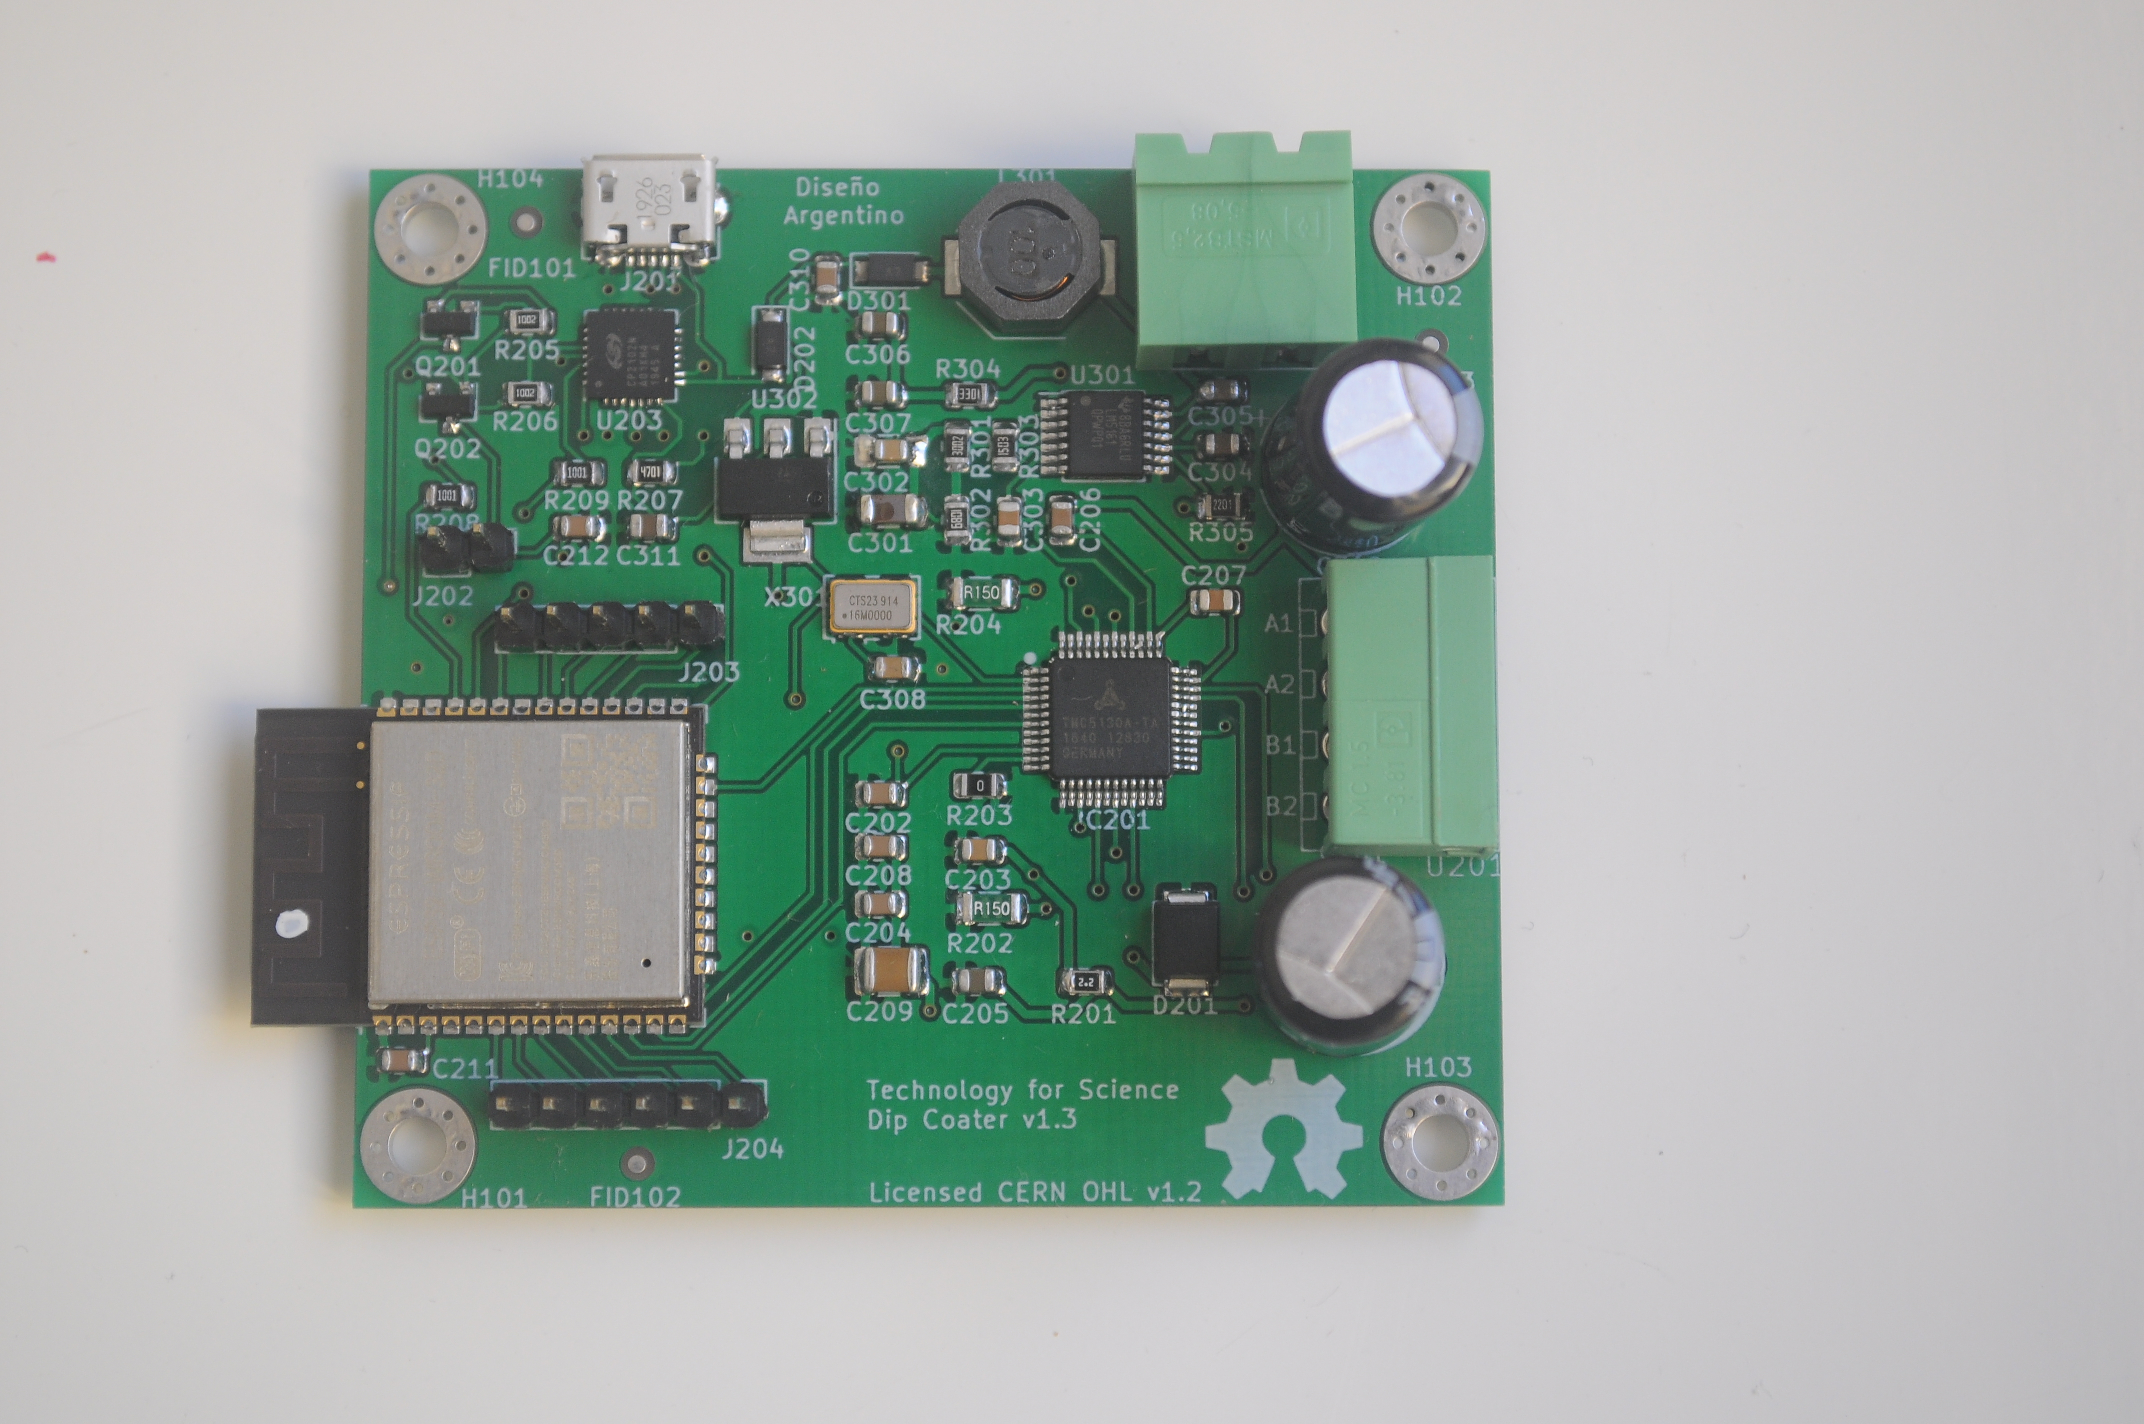
\includegraphics[width=.5\textwidth]{./Figures/dip_real_model.pdf}
	\caption{Placa fabricada MAYER SRL.}
	\label{fig:dip_real_model}
\end{figure}

  
%-----------------------------------
%	SUBSECTION 1
%-----------------------------------
\subsection{Diseño y fabricación}
%-----------------------------------
%	SUBSECTION 2
%-----------------------------------


%----------------------------------------------------------------------------------------
%	SECTION 2
%----------------------------------------------------------------------------------------

\section{Firmware}

\subsection{Capas de abstracción}
\subsection{Framework de trabajo}
\subsection{Módulos principales}



%----------------------------------------------------------------------------------------
%	SECTION 3
%----------------------------------------------------------------------------------------

\section{Estructura mecánica}

\subsection{Modelos 3D}
\subsection{Fabricación de piezas personalizadas a través de mecanizado CNC}


